\documentclass{../template/tp}
\usepackage[utf8x]{inputenc}

\usepackage[english]{babel}
\usepackage[T1]{fontenc}

\usepackage{graphicx}
\usepackage{amssymb}
\usepackage{amsmath}
\usepackage{wasysym} %smiley
\usepackage{hyperref}% hyperliens
\usepackage{tikz}
\usetikzlibrary{babel,positioning,calc}
\usepackage[]{circuitikz}
\usepackage{textcomp}
% \usepackage{minted}
\usepackage[long]{datetime}
\usepackage{gensymb} % \ohm, celsius
\usepackage{framed}
\usepackage{pdfpages}
\usepackage{todonotes}
\usepackage{enumitem}
\usepackage{ marvosym }
\usepackage{qrcode}%Don't forget to escape the "#", as the href package requires.
\usepackage{tabularx}

\usepackage{mathastext} % math as standfard text : units are respecting typography conventions.
\usepackage{fancyhdr}
% \langexam{frenchb}

\usepackage{subcaption}

\graphicspath{{imgs/}}

\newcommand{\labTitle}{GRAFCET}
\newcommand{\labNumber}{3}

\newcommand{\version}{v1.0.0}

\newcommand{\mnemonic}{ELEC-H-516}
\newcommand{\courseName}{Programmable Logic Controllers}

\newboolean{koriG}
\ifx\koriG\undefined
\correction{false}
\else
\correction{true}
\fi

% \correction{false}
% \correction{true}

\author{The Fantastic Four}


%% fancy header & foot
\pagestyle{fancy}
\lhead{[\mnemonic] \courseName\\ LABO  \labNumber :  \labTitle}
\rhead{\version\\ page \thepage}
\cfoot{}
%%

\pdfinfo{
/Author (ULB -- BEAMS)
/Title (Labo \labNumber \mnemonic, \labTitle)
/ModDate (D:\pdfdate)

}
\hypersetup{
pdftitle={Labo \labNumber [\mnemonic] \courseName : \labTitle},
pdfauthor={©2017 ULB - BEAMS  },
pdfsubject={\labTitle}
}


\setlength{\parskip}{0.5cm plus4mm minus3mm} %espacement entre §
\setlength{\parindent}{0pt}

\begin{document}

\tptitle{}{Labo \labNumber : \labTitle}

\vspace{-1cm}

\rule{\linewidth}{.5pt}

\Question{
	The process is described as follows: product A is first weighted until the balance reaches the point a, and then is placed in the reservoir. The same procedure is repeated for product B. After the product B is placed in the reservoir, 2 solid blocks of the product D are placed in
	the reservoir. When all three products are in the reservoir the valve C has been opened to provide liquid to the reservoir. The amount of the liquid is controlled by the time the valve is opened (or until given level is reached). Once the liquid is in the mixer will steer everything for 30s. The reservoir is emptied and the system is ready to start a new sequence.
	
	Build the SFC that controls the process described above and provide the necessary simulation environment.
	
	\begin{figure}[h]
		\centering
		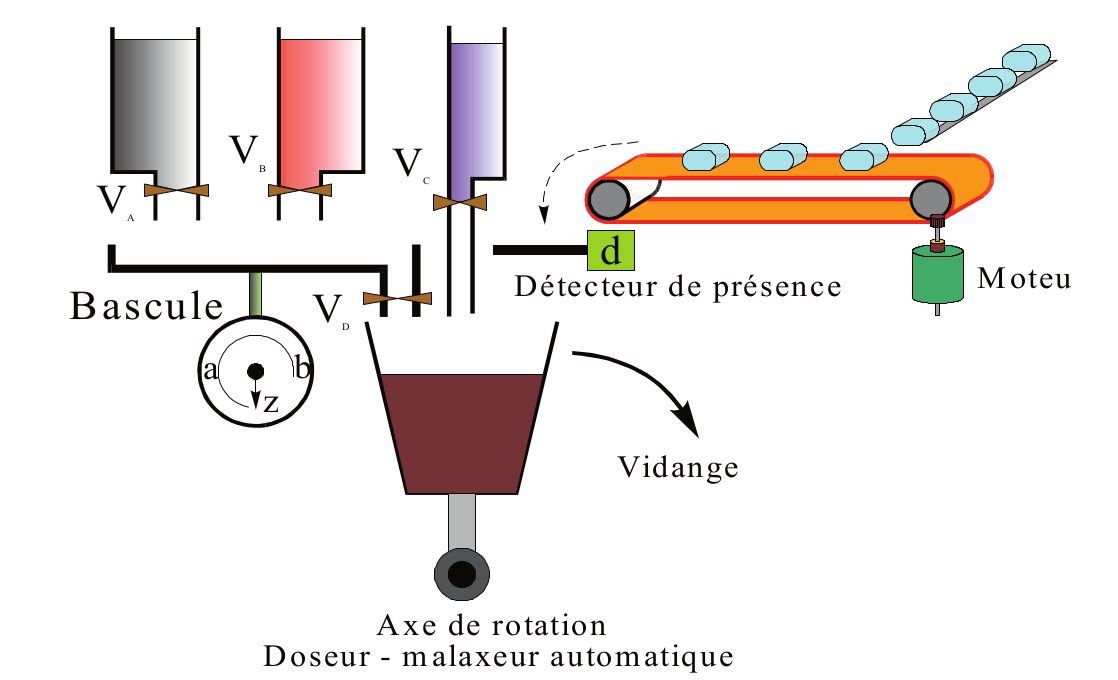
\includegraphics[width=0.8\linewidth]{exo1}
		\caption{}
		\label{grafcet}
	\end{figure}

}{}

\newpage

\Question{
	Imagine a wagon in the position $ A_{1} $ where he needs to pick-up some useful load. When the wagon gets the load, he can go to the position $ B_{1} $ to discharge the load. This process is controlled with the bouton $ d_{A1} $. Immediately after the loading is complete, the wagon moves towards the position $ B_{1} $, to disembark the load. If the disembark position is free, wagon should move forward to the positions $ C $, to actually discharge the load. Once the load is off, the wagon moves back to the position $ A_{1} $. Note that if for some reason the position $ C $ is occupied (not free), the wagon should wait in $ B_{1} $.

	The disembarking position $ C $ is common for few wagons that can pick-up the load at different positions and discharge it at the same position $ C $. For this exercise consider the case of two wagons (the second one being marked with $ A_{2} $).

	Build the SFC that controls the process described above and provide the necessary simulation environment.
	
	\begin{figure}[h]
		\centering
		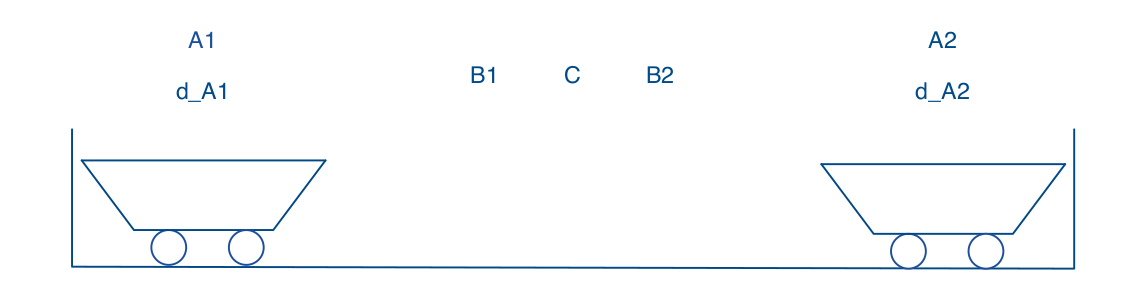
\includegraphics[width=0.8\linewidth]{exo2}
		\caption{}
		\label{grafcet}
	\end{figure}
}{}


\end{document}